% !TEX TS-program = pdflatex
% !TEX encoding = UTF-8 Unicode

% This is a simple template for a LaTeX document using the "article" class.
% See "book", "report", "letter" for other types of document.

\documentclass[12pt]{article} % use larger type; default would be 10pt

\usepackage[utf8]{inputenc} % set input encoding (not needed with XeLaTeX)

\usepackage{kotex}

%%% Examples of Article customizations
% These packages are optional, depending whether you want the features they provide.
% See the LaTeX Companion or other references for full information.

%%% PAGE DIMENSIONS
\usepackage{geometry} % to change the page dimensions
\geometry{a4paper} % or letterpaper (US) or a5paper or....
% \geometry{margin=2in} % for example, change the margins to 2 inches all round
% \geometry{landscape} % set up the page for landscape
%   read geometry.pdf for detailed page layout information

\usepackage{graphicx} % support the \includegraphics command and options

% \usepackage[parfill]{parskip} % Activate to begin paragraphs with an empty line rather than an indent

%%% PACKAGES
\usepackage{booktabs} % for much better looking tables
\usepackage{array} % for better arrays (eg matrices) in maths
\usepackage{paralist} % very flexible & customisable lists (eg. enumerate/itemize, etc.)
\usepackage{verbatim} % adds environment for commenting out blocks of text & for better verbatim
\usepackage{subfig} % make it possible to include more than one captioned figure/table in a single float

\usepackage{makeidx}
\usepackage{titling}
\usepackage{indentfirst}

% These packages are all incorporated in the memoir class to one degree or another...

%%% HEADERS & FOOTERS
\usepackage{fancyhdr} % This should be set AFTER setting up the page geometry
\pagestyle{fancy} % options: empty , plain , fancy
\renewcommand{\headrulewidth}{0pt} % customise the layout...
\lhead{}\chead{}\rhead{}
\lfoot{}\cfoot{\thepage}\rfoot{}

%%% SECTION TITLE APPEARANCE
\usepackage{sectsty}
% \allsectionsfont{\sffamily\mdseries\upshape} % (See the fntguide.pdf for font help)
% (This matches ConTeXt defaults)

%%% ToC (table of contents) APPEARANCE
\usepackage[nottoc,notlof,notlot]{tocbibind} % Put the bibliography in the ToC
\usepackage[titles,subfigure]{tocloft} % Alter the style of the Table of Contents
\renewcommand{\cftsecfont}{\rmfamily\mdseries\upshape}
\renewcommand{\cftsecpagefont}{\rmfamily\mdseries\upshape} % No bold!

%%% ADDITIONAL %%%

\pagenumbering{gobble}
\renewcommand{\thesection}{\Roman{section}} 
\setlength{\parindent}{1cm}
\overfullrule=2cm



%%% BIBLIOGRAPHY %%%




%%% END Article customizations

%%% The "real" document content comes below...

\title{Separation of R- and S- Etodolac Enantiomers by High Performance Liquid Chromatography - Florence Detector after Derivatization with (1R)-(-)-Menthyl Chloroformate}
\author{Hanpil Kang}
\date{} % Activate to display a given date or no date (if empty),
         % otherwise the current date is printed 
\makeindex
\begin{document}






\setcounter{page}{1}
\pagenumbering{roman}

\maketitle

\begin{abstract}
Etodolac, one of nonsteroidal anti-inflammatory drugs(NSAIDs) found in R/S- form are shown to be have different pharmacodynamic and pharmacokinetic properties. R- contreats Leukemia while S- treats the symptoms of pain and inflammation. In this research, (1R)-(-)-Menthyl Chloroformate was used to derivate R/S- Etodolac which reacts with the Carboxyl group in pyridine catalyst. High Performance Liquid Chromatography - Florence Detector (HPLC-FLD) and Ultra Performance Liquid Chromatography - Mass Detector (UPLC-MS) with reverse phased columns are used to qualificate two enantiomers of Etodolac. Two peaks appears at 13.115 and 14.196 in HPLC-FLD. First peak is R-Etodolac derivatizated with (1R)-(-)-Menthyl Chloroformate while the other one is S-Etodolac. Resolution is over 1 in both standard and serum sample.  
\end{abstract}

\newpage

한글초록

\newpage

\tableofcontents

\newpage

\listoffigures

\newpage

\listoftables

\newpage



\setcounter{page}{1}
\pagenumbering{arabic}

\section{Introduction}

Etodolac, one of the nonsteroidal anti-inflamatory drugs (NSAIDs) is widely used for treating rheumatic and inflammatory diseases. This drug is used in the form of a racemic mixture but the pharmacodynamic and pharmacokinetic properties of the two enantimoers are different. R- contreats Leukemia\cite{cite1} while S- treats symptoms like pain and inflammation. Menthyl Chloroformate was widely used as a derivating secondary amine, but it also reacts with the carboxyl group when the catalyst pyridine exists.
High Performance Liquid Chromatography – Florence Detector (HPLC-FLD) and Ultra Performance Liquid Chromatography – Mass spectrometry (UPLC-MS) are powerful machines which can quantify and qualify products. 
In this research, HPLC-FLD was used to detect products made by the derivatization of (1R)-(-)-Menthyl Chloroformate to Etodolac. To check the two isomers' structure, UPLC-MS was used.


\begin{figure}[h]
  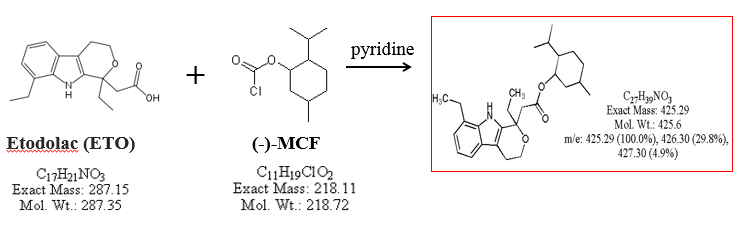
\includegraphics[width=\linewidth]{fig1.png}
  \caption{Etodolac, (-)-MCF and their products.}
  \label{fig:fig1}
\end{figure}

\newpage




\section{Experimental}

\subsection{Chemicals and Reagents}
  R/S-Etodolac was purchased from Tokyo Chemical Industry (Tokyo, Japan).
  (1R)-(-)-Menthyl Chloroformate, Pyridine, L-Proline was purchased from Sigma-Aldrich Chemie (St. Louis, USA).
  Acetonitrile (ACN) and Methanol (MeOH) were purchased from Avantor Performance Materials, Inc (USA).
NaCl was purchased from Merck KGaA (Darmstadt, Germany).

\subsection{High-performance Liquid Chromatography - Florence Detector}
  High-performance liquid chromatography (HPLC) is widely used in analytic chemistry to separate, identify or quantify each component in a mixture. Gemini C18 Column was used at a flow rate of 1.0mL/min at 25$^{\circ}$C  used with 86.5\% MeOH, 13.5\% 10mM Acetic Acid.
  Florence Detector was used at a wavelength of $\lambda$ex= 235 nm; $\lambda$ em= 345 nm.

  Chemstation Software was used for system control and data processing.


\subsection{Ultra-performance liquid chromatography – Mass Detector}

  Ultra-performance liquid chromatography – Mass Spectrometer (UPLC-MS) is widely used in analytic chemistry to separate, identify or quantify each component in a mixture through mass detection. A mass spectrum is a plot of the ion signal as a function of the mass-to-charge ratio. Mass spectra are used to determine the elemental or isotopic signature of a sample, find the masses of particles and of molecules, and to elucidate the chemical structures of molecules, such as peptides and other chemical compounds. UPLC BEH C18 Column (2.1 x 50mm, 1.7um) was used at a flow rate of 0.3mL/min, at 45$^{\circ}$C. Elution conditons can be seen in [Table \ref{tab:table1}]. MassLynx Software was used for system control and data processing.

\begin{table}[h]
  \begin{center}
    \caption{Elution Condition of UPLC-MS.}
    \label{tab:table1}
    \begin{tabular}{ccc}
      \toprule
      Time(min) & Water(0.1\% Formic Acid) & Methanol (0.1\% Formic Acid) \\
      \midrule
      0 & 20 & 80 \\
      \midrule
      9 & 10 & 90 \\
      \midrule
      11 & 0 & 100 \\
      \midrule
      13 & 0 & 100 \\
      \midrule
      15 & 20 & 80 \\
      \midrule
      17 & 20 & 80 \\
      \bottomrule
    \end{tabular}
  \end{center}
\end{table}

\subsection {Protocol}
 The protocol for this experiment was as follows. 50uL 50mM etodolac soluted in ACN was added to 50uL urine. The solution was vortexed for 3 seconds, and then 900uL of ACN was added. The solution was then vortexed for 3 minutes, and then centrifuged for 5 minutes at 13500 rounds per minute. Next, 950uL of the upper layer of the solution was moved to another vial and evaporated using gentle nitorgen stream at 40 $^{\circ}$C After, 160uL 100mM MCF soluted in ACN, 15uL pyridine, 25uL ACN were all added to the residue, and it was sonicated for 10 inutes. To finalize derivatization, 160uL 100mM proline soluted in distilled water was added, and then vortexed for 3 minutes. After being vortesed, it was placed at room temperature for 20 minutes. 28.7 mg of NaCl was added for Liquid-Liquid Extraction and the organic layer was filtered to complete to the optimization process.


\subsection {In-vitro test}
 S-etodolac binds well to Albumin than R-etodolac.\cite{cite4} Etodolac enantiomers were attempted to be identified using the stereoselective binding difference of etodolac to albumin.
 Protocol follows.  Add 100uL 50ppm Etodolac. Evaporate in 40'C in gentle nitrogen stream. Add 100uL 50ppm Albumin in pH 7.4 phosphate buffer.
 Albumin purification was done to separate unbound Etodolac. We used Vivaspin 500 to separate protein.
 Protocol follows. In Vivaspin 500 add 100uL diluted water and centrifuge in 10000g for 5 minute. Add 100uL albumin and Etodolac mixture and centrifuge in 10000g for 3 minute. Filter 50uL and add 100 uL buffer and centrifuge in 10000g for 5minute. Repeat 4 times filtering 100uL and adding 100uL buffer and centrifuge in 100g for 5minute. Transfer concentrate and collect filtrate.


\subsection {In-vivo test for rats}
 C57BL/6 mouse (male; 7 w) serum was used for Chrial determination of \linebreak etodolac. The weight of mouse was 20g. Concentration of S-(+)-etodolac is lower than R-(-)-etodolac when injected 20mg/kg from 0 through 70 hour.\cite{cite2}
  Protocol follows. Add 10mg etodolac to 50uL ethanol and vortex for 20s. Add 300uL Tween 80 and vortex for 1 minute and sonicate for 1 minute. After centrifuging 3 seconds, add saline to 10mL. Inject etodolac to mouse.
  200uL was injected to C57 mouse when the weight was 20g.


  

\newpage

\section {Results and Discussion}

\subsection {UPLC-MS Data}


\begin{figure}[h]
  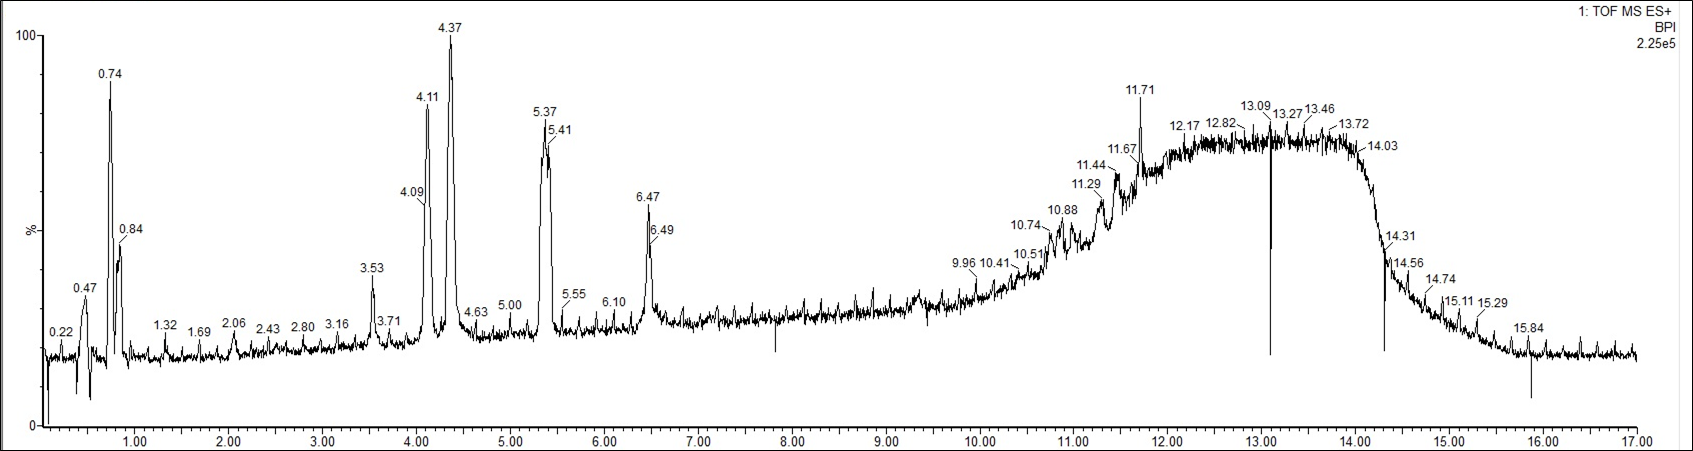
\includegraphics[width=\linewidth]{bpi.png}
  \caption{BPI chromatogram of Menthyl Chloroformate-derivatized Etodolac product }
  \label{fig:fig2}
\end{figure}
\begin{figure}[h]
  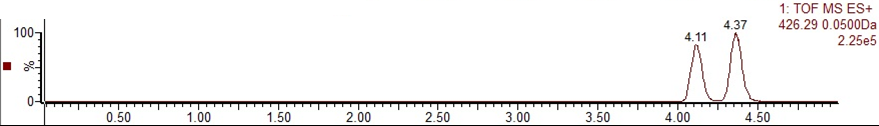
\includegraphics[width=\linewidth]{fig3.png}
  \caption{Extract ion chromatogram of Menthyl Chloroformate-derivatized Etodolac product, [M+H]=426.29}
  \label{fig:fig3}
\end{figure}
\begin{figure}[h!]
  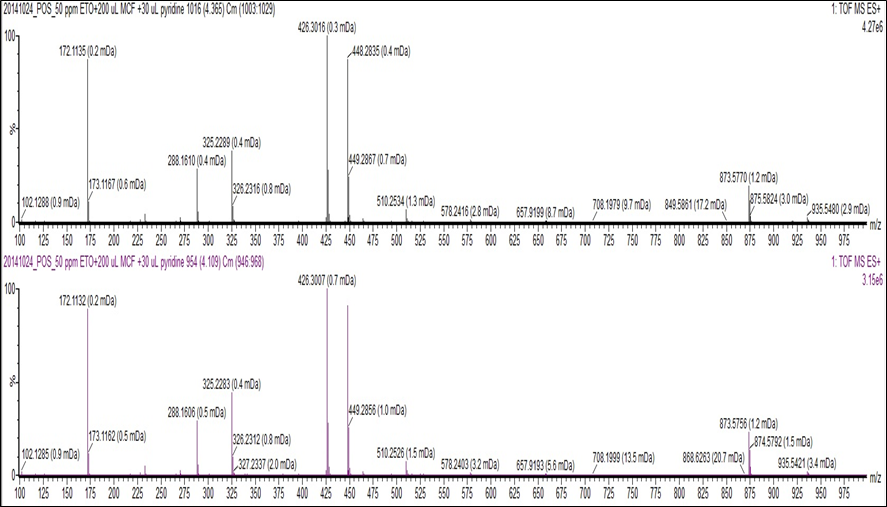
\includegraphics[width=\linewidth]{fig4.png}
  \caption{Mass fragment of peak at retention time 4.11 minute and 4.37 minute.}
  \label{fig:fig4}
\end{figure}

In [Figure \ref{fig:fig4}], the mass fragment of the peak at 4.11 and 4.37 are equal. This means they are not geometric isomers, but they appear at different peaks. The mass at 172.1 and 287.15 shows that they have the structure of an etodolac.\cite{cite3} So it can concluded that they are derivated etodolac. 


\subsection {HPLC-FLD Data}
\begin{figure}[h!]
  \centering
  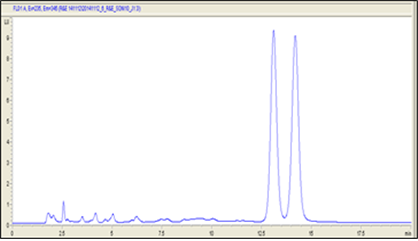
\includegraphics[width=\linewidth]{fig5.png}
  \caption{HPLC-FLD data of protocol}
  \label{fig:fig5}
\end{figure}

 In [Figure \ref{fig:fig5}], two peaks appear at 13.115 and 14.196. Two are enantiomers of etodolac derivatized by Menthyl Chlroforomate. The first peak will be referred to as Peak 1, and the second, Peak 2.

\subsection{ Protocol Optimization }
 The Pyridine volume and sonication time was optimized in this experiment. Peak 2 reacted faster than Peak 1. Therefore, the ratio of Peak 1 was used to verify that the reaction was completed.

\subsubsection {Pyridine Volume}


\begin{figure}[h!]
  \centering
  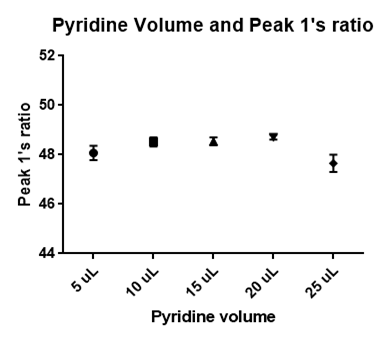
\includegraphics[width=0.6\linewidth]{fig6.png}
  \caption{Pyridine Volume and Peak 1's ratio}
  \label{fig:fig6}
\end{figure}

 In [Figure \ref{fig:fig6}],  5uL and 25uL of pyridine volume were significant by t-test. Optimized value found to be the median of the pyridine volume, which was not significant, 15uL.

\subsubsection {Sonication time}

\begin{figure}[h!]
  \centering
  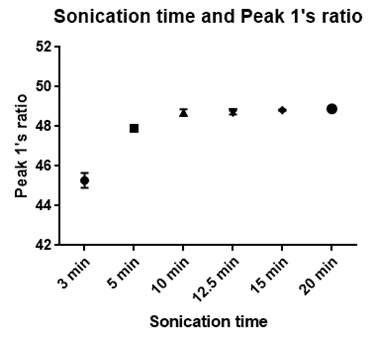
\includegraphics[width=0.6\linewidth]{fig7.png}
  \caption{Sonication time and Peak 1's ratio}
  \label{fig:fig7}
\end{figure}
  In [Figure \ref{fig:fig7}],  3min and 5min of sonication time were significant by t-test. Optimized value found to be the first of the significant time, which was not significant, 10min.



\subsection {In-vitro test}
\begin{figure}[h!]
  \centering
  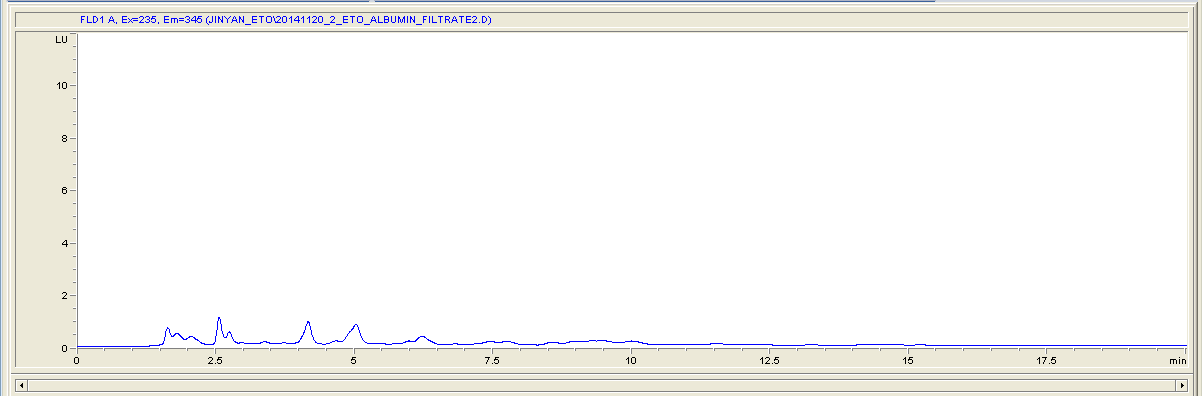
\includegraphics[width=\linewidth]{fig8.png}
  \caption{Chromatogram of Filtrate}
  \label{fig:fig9}
\end{figure}
 The in vitro test failed beacuse both etodolac enantiomers were well binded with protein in a short time, so the results of in-vivo test were analyzed.

\subsection {In-vivo test for rats}

\begin{figure}[h!]
  \centering
  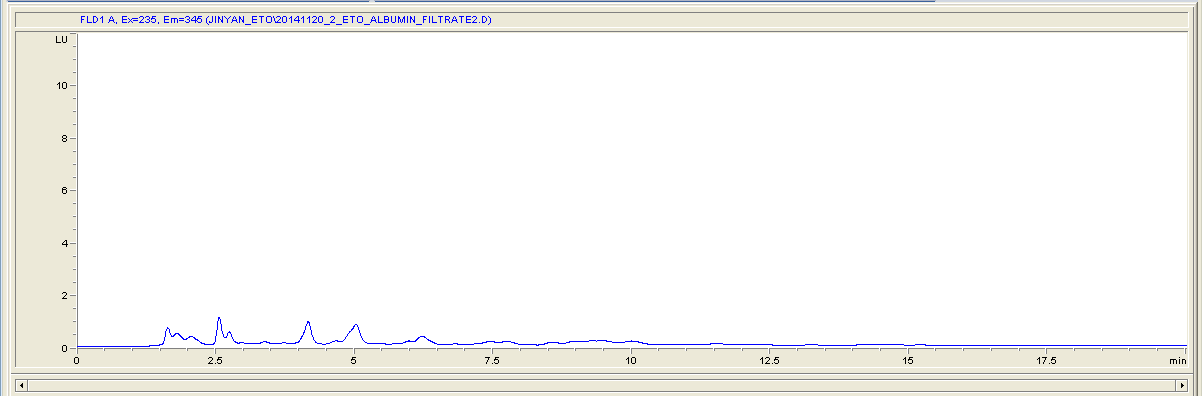
\includegraphics[width=\linewidth]{f9.png}
  \caption{In vivo test result}
  \label{fig:fig8}
\end{figure}

 In [Figure \ref{fig:fig8}],  1 hour after injection, the peak area of Peak 1 is 0.4676, while the peak area of Peak 2 is 0.0694. S-etodolac binds faster\cite{cite2} and Peak 2 has less peak area, which means that Peak 2 is S-etodolac and Peak 1 is R-etodolac.



\newpage

\begin{thebibliography}{100}
\bibitem{cite1}
	Brocks, D. R., Jamali, F., J. Pharm. Sci. 1991, 80, 1058– 1061.


\bibitem{cite2}
        Shi JM et al. / Aeta Pharmacol Sin 2004 Aug; 25 (8): 996-999

\bibitem{cite3}
        Clin Pharmacokinet. Joseph P. Boni, Joan M. Korth-Bradely, Lyette S. Richards, Soong T Chiang, David R. Hicks, Leslie Z. Benet. 2000 Dec, 39(6) 459-469

\bibitem{cite4}
	Chang-Chuan Guo et al. / Journal of Pharmaceutical Analysis  2011;1(3):184-190

\end{thebibliography}

























\end{document}
